\PassOptionsToPackage{dvipsnames,svgnames,x11names}{xcolor}
\documentclass[landscape,a0paper,fontscale=0.32]{baposter}

% For graphs
\usepackage{graphicx}

\usepackage{array}
\usepackage{booktabs}
\usepackage{eso-pic}
\usepackage{layout}
\usepackage{fancybox}


\usepackage{calc}
\usepackage{amsmath}
\usepackage{amssymb}
\usepackage{relsize}
\usepackage{multirow}
\usepackage{rotating}
\usepackage{bm}
\usepackage{url}
\usepackage{xfrac}
\usepackage{natbib}
\usepackage{mathtools}
\usepackage{cancel}
\usepackage{paralist}
\usepackage{nicefrac}
\usepackage[export]{adjustbox} % loads also graphicx
\usepackage{caption}
\usepackage{xfrac}

% \usepackage[centering,includeheadfoot,margin=2cm]{geometry}

\usepackage{multicol}

% \usepackage[linesnumbered,ruled,vlined,noend]{algorithm2e}
% % \usepackage{algorithmicx}
% % \usepackage{algpseudocode}
% \newlength\figureheight
% \newlength\figurewidth
% \setlength{\algomargin}{2em}
% \SetKwComment{Comment}{$\blacktriangleright$\ }{}
% 
% \providecommand{\SetAlgoLined}{\SetLine}
% \providecommand{\DontPrintSemicolon}{\dontprintsemicolon}

\newcommand{\figurewidth}{7cm}
\newcommand{\figureheight}{3cm}

%\usepackage{times}
%\usepackage{helvet}
%\usepackage{bookman}
\usepackage{palatino}

%\newcommand{\captionfont}{\footnotesize}

\usetikzlibrary{calc}

% \newcommand{\SET}[1]  {\ensuremath{\mathcal{#1}}}
% \newcommand{\MAT}[1]  {\ensuremath{\boldsymbol{#1}}}
% \newcommand{\VEC}[1]  {\ensuremath{\boldsymbol{#1}}}
% \newcommand{\Video}{\SET{V}}
% \newcommand{\video}{\VEC{f}}
% \newcommand{\track}{x}
% \newcommand{\Track}{\SET T}
% \newcommand{\LMs}{\SET L}
% \newcommand{\lm}{l}
% \newcommand{\PosE}{\SET P}
% \newcommand{\posE}{\VEC p}
% \newcommand{\negE}{\VEC n}
% \newcommand{\NegE}{\SET N}
% \newcommand{\Occluded}{\SET O}
% \newcommand{\occluded}{o}

\renewcommand{\sfdefault}{lmss}
\sffamily

\newcommand{\listhead}[1] {\textsc{\underline{#1}}}

\definecolor{rouge1}{RGB}{226,0,38}  % red P
\definecolor{orange1}{RGB}{243,154,38}  % orange P
\definecolor{jaune}{RGB}{254,205,27}  % jaune P
\definecolor{blanc}{RGB}{255,255,255} % blanc P

\definecolor{rouge2}{RGB}{230,68,57}  % red S
\definecolor{orange2}{RGB}{236,117,40}  % orange S
\definecolor{taupe}{RGB}{134,113,127} % taupe S
\definecolor{gris}{RGB}{91,94,111} % gris S
\definecolor{bleu1}{RGB}{38,109,131} % bleu S
\definecolor{bleu2}{RGB}{28,50,114} % bleu S
\definecolor{vert1}{RGB}{133,146,66} % vert S
\definecolor{vert3}{RGB}{20,200,66} % vert S
\definecolor{vert2}{RGB}{157,193,7} % vert S
\definecolor{darkyellow}{RGB}{233,165,0}  % orange S
\definecolor{lightgray}{rgb}{0.9,0.9,0.9}
\definecolor{darkgray}{rgb}{0.6,0.6,0.6}

\definecolor{blue900}{HTML}{0D47A1}
\definecolor{blue800}{HTML}{1565C0}

\definecolor{green1}{RGB}{217,255,250}
\definecolor{orange1}{RGB}{250,245,217}

\newcommand{\rcol}[1]{\textcolor{red}{\textit{#1}}}
\newcommand{\gcol}[1]{\textcolor{vert3}{\textit{#1}}}
\newcommand{\bcol}[1]{\textcolor{blue}{\textit{#1}}}
\newcommand{\ycol}[1]{\textcolor{darkyellow}{\textit{#1}}}

\newcommand{\rcolb}[1]{\textcolor{red}{\textit{\textbf{#1}}}}
\newcommand{\gcolb}[1]{\textcolor{vert3}{\textit{\textbf{#1}}}}
\newcommand{\bcolb}[1]{\textcolor{blue}{\textit{\textbf{#1}}}}
\newcommand{\ycolb}[1]{\textcolor{darkyellow}{\textit{\textbf{#1}}}}

\newcommand{\otoprule}{\midrule[\heavyrulewidth]}
\newcommand{\dbacks}[1]{\textbf{\textcolor{red!80!black}{{#1}}}}

\colorlet{redp}{red!20} % vert S
\colorlet{greenp}{vert3!20} % vert S\usepackage[framemethod=tikz]{mdframed}
\colorlet{bluep}{blue!12} % vert S
\colorlet{blueg}{blue!70!green!90!white}
\definecolor{yellowp}{rgb}{0.99, 0.99, 0.59}
\colorlet{orangep}{orange!40}
\newcommand{\hl}[3][\fboxsep1pt]{{#1\colorbox{#2}{#3}}}%
%\newcommand{\hl}[2]{{\adjustbox{bgcolor=#1}{#2}}}%

\newcommand{\hlr}[1]{\hl{redp}{#1}}
\newcommand{\hlg}[1]{\hl{greenp}{#1}}
\newcommand{\hlb}[1]{\hl{bluep}{#1}}
\newcommand{\hlo}[1]{\hl{orangep}{#1}}
\newcommand{\hly}[1]{\hl{yellow!70!black!40!white}{#1}}
\newcommand{\hlblg}[1]{\hl{blue!75!green!20!white}{#1}}
\newcommand{\tikzhlblg}[1]{\tikz[baseline]{\node[inner sep=2pt, anchor=base,fill=blue!75!green!20!white]{{#1}};}}
\newcommand{\tikzhly}[1]{  \tikz[baseline]{\node[inner sep=2pt, anchor=base,fill=yellow!70!black!50!white]{{#1}};}}
\newcommand{\tikzhlr}[1]{  \tikz[baseline]{\node[inner sep=2pt, anchor=base,fill=redp]{{#1}};}}
\newcommand{\tikzhlg}[1]{  \tikz[baseline]{\node[inner sep=2pt, anchor=base,fill=greenp]{{#1}};}}
\newcommand{\tikzhlb}[1]{  \tikz[baseline]{\node[inner sep=2pt, anchor=base,fill=bluep]{{#1}};}}

\usepackage{tikz,pgfplots}
\pgfplotsset{compat=newest}
\tikzstyle{every picture}+=[remember picture]
\tikzstyle{na} = [baseline=-.5ex]
\everymath{\displaystyle}
\usetikzlibrary{arrows,shapes}
\usetikzlibrary{positioning}

\usepackage{wasysym}

%\usepackage{tcolorbox}

\usepackage{algorithm}
\usepackage{algorithmic}

\usepackage{multirow}

\usepackage{tabu}

\usepackage{xspace}
\DeclareRobustCommand{\eg}{e.g.,\@\xspace}
\DeclareRobustCommand{\ie}{i.e.,\@\xspace}
\DeclareRobustCommand{\wrt}{w.r.t.\@\xspace}
\DeclareRobustCommand{\wp}{w.p.\@\xspace}

%=============================================
% General commands
%---------------------------------------------
\newcommand{\transpose}[1]{{#1}^\texttt{T}}
\DeclareMathOperator*{\EV}{\mathbb{E}}
\DeclareMathOperator*{\argmax}{\arg\,\max}
\DeclareMathOperator*{\argmin}{\arg\,\min}
\DeclareMathOperator*{\arginf}{\arg\,\inf}
\newcommand{\EVV}[2][x]{\EV_{#1}\left[{#2}\right]}
\newcommand{\norm}[2][\infty]{\left\|#2\right\|_{#1}}
\newcommand{\indfun}[1]{\mathds{1}\left(#1\right)}

\newcommand{\realspace}{\mathbb R}		% realspace
\newcommand{\natspace}{\mathbb N}		% naturalspace
\newcommand{\pdfunc}[1]{p\left(#1\right)}	% density function
\newcommand{\prob}[1]{Pr\left(#1\right)}	% probability
\newcommand{\funoper}[1]{\left[#1\right]}	% function operator
\newcommand{\apx}[1]{\widetilde{#1}}		% approximation symbol
\newcommand{\e}{\boldsymbol{e}} 		% unit vector

\newcommand{\texsub}[1]{\textsc{\tiny #1}}


%=============================================
% RL Commands
%---------------------------------------------
%%% MDPs
\newcommand{\mdp}{\mathcal{M}}				% MDP
\newcommand{\statespace}{\mathcal S}			% state space
\newcommand{\actionspace}{\mathcal A}			% action space
\newcommand{\pmodel}{\mathcal P}			% transition function
\newcommand{\pmodelfun}[1]{\pmodel\left(#1\right)}	% transition function
\newcommand{\rmodel}{\mathcal R}			% reward function
\newcommand{\rmodelfun}[1]{\rmodel\left(#1\right)}	% reward function
\newcommand{\initD}{\mu}					% initial distribution

%% Policy Gradient
\newcommand{\vtheta}{\boldsymbol{\theta}}
\newcommand{\gradJ}[1]{\nabla J({#1})}
\newcommand{\vphi}{\boldsymbol{\phi}}
\newcommand{\DeltaJ}{J(\vtheta') - J(\vtheta)}
\newcommand{\gradApp}[1]{\widehat{\nabla}_{#1}J(\vtheta)}
\newcommand{\gradSim}[1]{\tilde{\nabla}_{#1}J(\vtheta)}
\newcommand{\gradRF}[1]{\hat{\nabla}_{#1}J^{RF}(\vtheta)}
\newcommand{\gradPGT}[1]{\hat{\nabla}_{#1}J^{PGT}(\vtheta)}
\newcommand{\gradGPOMDP}[1]{\hat{\nabla}_{#1}J^{G(PO)MDP}(\vtheta)}
\newcommand{\gradDown}[1]{\underline{\hat{\nabla}_{#1}J}(\vtheta)}
\newcommand{\gradUp}[1]{\overline{\hat{\nabla}_{#1}J}(\vtheta)}

%Specific
\newcommand{\Ets}[2][t]{\mathbb{E}_{#1\vert s}\left[#2\right]}
\newcommand{\Es}[1]{\mathbb{E}_{s}\left[#1\right]}
\newcommand{\Covts}[3][t]{{\mathbb{C}\text{ov}}_{#1\vert s}\left(#2,#3\right)}
\newcommand{\Covs}[2]{{\mathbb{C}\text{ov}}_{s}\left(#1,#2\right)}
\newcommand{\Var}[1]{{\mathbb{V}\text{ar}}\left[#1\right]}
\newcommand{\Varts}[2][t]{{\mathbb{V}\text{ar}}_{#1\vert s}\left[#2\right]}
\newcommand{\Vars}[1]{{\mathbb{V}\text{ar}}_{s}\left[#1\right]}
\newcommand{\gradBlack}[1]{\blacktriangledown J(#1)}
\newcommand{\gradIdeal}[1]{\dnabla J(#1)}
\newcommand{\VARRF}{V}
\newcommand{\GRADLOG}{G}
\newcommand{\VARIS}{W}
\newcommand{\HESSLOG}{F}
% short forms 
\newcommand{\wt}[1]{\widetilde{#1}}
\newcommand{\wh}[1]{\widehat{#1}}
\newcommand{\wo}[1]{\overline{#1}}
\newcommand{\wb}[1]{\overline{#1}}

%Colors
\definecolor{crimson}{rgb}{0.86, 0.08, 0.24}
\definecolor{myblue}{rgb}{0.0, 0.44, 1.0}
\definecolor{amber2}{rgb}{1.0, 0.49, 0.0}
\newcommand{\chall}[1]{\textcolor{amber2}{\textbf{#1}}}
\newcommand{\bad}[1]{\textcolor{crimson}{\textbf{#1}}}
\newcommand{\enhance}[1]{\textcolor{myblue}{\textbf{#1}}}

%Fake items
\newcommand{\tabitem}[1]{~~\llap{\textbullet}~~ #1 \hfill\mbox{}}

%%%%%%%%%%%%%%%%%%%%%%%%%%%%%%%%%%%%%%%%%%%%%%%%%%%%%%%%%%%%%%%%%%%%%%%%%%%%%%%%
%%%% Some math symbols used in the text
%%%%%%%%%%%%%%%%%%%%%%%%%%%%%%%%%%%%%%%%%%%%%%%%%%%%%%%%%%%%%%%%%%%%%%%%%%%%%%%%

%%%%%%%%%%%%%%%%%%%%%%%%%%%%%%%%%%%%%%%%%%%%%%%%%%%%%%%%%%%%%%%%%%%%%%%%%%%%%%%%
% Multicol Settings
%%%%%%%%%%%%%%%%%%%%%%%%%%%%%%%%%%%%%%%%%%%%%%%%%%%%%%%%%%%%%%%%%%%%%%%%%%%%%%%%
\setlength{\columnsep}{1.5em}
\setlength{\columnseprule}{0mm}

%%%%%%%%%%%%%%%%%%%%%%%%%%%%%%%%%%%%%%%%%%%%%%%%%%%%%%%%%%%%%%%%%%%%%%%%%%%%%%%%
% Save space in lists. Use this after the opening of the list
%%%%%%%%%%%%%%%%%%%%%%%%%%%%%%%%%%%%%%%%%%%%%%%%%%%%%%%%%%%%%%%%%%%%%%%%%%%%%%%%
\newcommand{\compresslist}{%
\setlength{\itemsep}{1pt}%
\setlength{\parskip}{0pt}%
\setlength{\parsep}{0pt}%
}

\captionsetup{justification=raggedright,singlelinecheck=false}


% box for algorithms
\newlength{\minipagewidth}
\newlength{\minipagewidthx}
\setlength{\minipagewidth}{0.99\textwidth}
\setlength{\minipagewidthx}{0.99\textwidth}
\setlength{\fboxsep}{1.5mm}
\addtolength{\minipagewidth}{-\fboxrule}
\addtolength{\minipagewidth}{-\fboxrule}
\addtolength{\minipagewidth}{-\fboxsep}
\addtolength{\minipagewidth}{-\fboxsep}
\addtolength{\minipagewidthx}{+\fboxsep}
\newcommand{\bookbox}[1]{
\par\medskip\noindent
\framebox[\columnwidth]{
\begin{minipage}{\minipagewidth} {#1} \end{minipage} } \par\medskip }

\newcommand{\bookboxx}[1]{\small
\par\medskip\noindent
\framebox[0.99\textwidth]{
\begin{minipage}{0.97\dimexpr\textwidth-\parindent\relax} {#1} \end{minipage} } \par\medskip }

%Reduce linespace in biblio
\setlength{\bibsep}{2pt}

\usepackage[many]{tcolorbox}
\usetikzlibrary{decorations.pathreplacing}
%\tcbset{%
%	enhanced,
%	coltitle=black, 
%	detach title,
%	left=10mm,
%	overlay={
%		\node[rotate=90, minimum width=1cm, anchor=south,yshift=-0.8cm] at (frame.east) {\tcbtitle};
%	}
%}
\newtcolorbox{rightbrace1}{%
	boxsep=0cm,
	left=.05cm,
	top=.05cm,
	bottom=.05cm,
	grow to left by=-.35cm,
	colback=black!10,
	enhanced jigsaw, 
	breakable, % allow page breaks
	frame hidden, % hide the default frame
	width=6.1cm,
	overlay={%
		\draw [
		fill=none, % fill paper
		decoration={brace,amplitude=0.5em},
		decorate,
		ultra thick,
		darkgray,
		]
		% right line
		(frame.north east)--(frame.south east);
		\node[rotate=270, minimum width=1cm, anchor=south,yshift=0.35cm] at (frame.east) {iteration};
	},
	% paragraph skips obeyed within tcolorbox
	parbox=false,
}
%
\newtcolorbox{rightbrace2}{%
	boxsep=0cm,
	left=.05cm,
	top=.05cm,
	bottom=.05cm,
	grow to left by=-.35cm,
	colback=black!5!white,
	enhanced jigsaw, 
	breakable, % allow page breaks
	frame hidden, % hide the default frame
	width=7.6cm,
	overlay={%
		\draw [
		fill=none, % fill paper
		decoration={brace,amplitude=0.5em},
		decorate,
		ultra thick,
		darkgray,
		]
		% right line
		(frame.north east)--(frame.south east);
		\node[rotate=270, minimum width=1cm, anchor=south,yshift=0.3cm] at (frame.east) {epoch};
	},
	% paragraph skips obeyed within tcolorbox
	parbox=false,
}

\usepackage{stackengine}
\usepackage{scalerel}
\newcommand\dangersign[1][2ex]{%
	\renewcommand\stacktype{L}%
	\scaleto{\stackon[1.5pt]{\color{crimson}$\triangle$}{\tiny \bfseries{!}}}{#1}%
}

%%%%%%%%%%%%%%%%%%%%%%%%%%%%%%%%%%%%%%%%%%%%%%%%%%%%%%%%%%%%%%%%%%%%%%%%%%%%%%
%%% Begin of Document
%%%%%%%%%%%%%%%%%%%%%%%%%%%%%%%%%%%%%%%%%%%%%%%%%%%%%%%%%%%%%%%%%%%%%%%%%%%%%%

\begin{document}

%%%%%%%%%%%%%%%%%%%%%%%%%%%%%%%%%%%%%%%%%%%%%%%%%%%%%%%%%%%%%%%%%%%%%%%%%%%%%%
%%% Here starts the poster
%%%---------------------------------------------------------------------------
%%% Format it to your taste with the options
%%%%%%%%%%%%%%%%%%%%%%%%%%%%%%%%%%%%%%%%%%%%%%%%%%%%%%%%%%%%%%%%%%%%%%%%%%%%%%
% Define some colors

%\definecolor{lightblue}{cmyk}{0.83,0.24,0,0.12}
\definecolor{lightblue}{rgb}{0.145,0.6666,1}

% % Draw a video
% \newlength{\FSZ}
% \newcommand{\drawvideo}[3]{% [0 0.25 0.5 0.75 1 1.25 1.5]
%    \noindent\pgfmathsetlength{\FSZ}{\linewidth/#2}
%    \begin{tikzpicture}[outer sep=0pt,inner sep=0pt,x=\FSZ,y=\FSZ]
%    \draw[color=lightblue!50!black] (0,0) node[outer sep=0pt,inner sep=0pt,text width=\linewidth,minimum height=0] (video) {\noindent#3};
%    \path [fill=lightblue!50!black,line width=0pt] 
%      (video.north west) rectangle ([yshift=\FSZ] video.north east) 
%     \foreach \x in {1,2,...,#2} {
%       {[rounded corners=0.6] ($(video.north west)+(-0.7,0.8)+(\x,0)$) rectangle +(0.4,-0.6)}
%     }
% ;
%    \path [fill=lightblue!50!black,line width=0pt] 
%      ([yshift=-1\FSZ] video.south west) rectangle (video.south east) 
%     \foreach \x in {1,2,...,#2} {
%       {[rounded corners=0.6] ($(video.south west)+(-0.7,-0.2)+(\x,0)$) rectangle +(0.4,-0.6)}
%     }
% ;
%    \foreach \x in {1,...,#1} {
%      \draw[color=lightblue!50!black] ([xshift=\x\linewidth/#1] video.north west) -- ([xshift=\x\linewidth/#1] video.south west);
%    }
%    \foreach \x in {0,#1} {
%      \draw[color=lightblue!50!black] ([xshift=\x\linewidth/#1,yshift=1\FSZ] video.north west) -- ([xshift=\x\linewidth/#1,yshift=-1\FSZ] video.south west);
%    }
%    \end{tikzpicture}
% }
% 
% \hyphenation{resolution occlusions}
% %%
\begin{poster}%
  % Poster Options
  {
  % Show grid to help with alignment
  columns=4,
  grid=false,
  % Column spacing
  colspacing=1em,
  % Color style
  bgColorOne=white,
  bgColorTwo=white,
  borderColor=blue900,
  headerColorOne=blue800,
  headerColorTwo=blue800,
  headerFontColor=white,
  boxColorOne=white,
  boxColorTwo=lightblue,
  % Format of textbox
  textborder=roundedleft,
  % Format of text header
  eyecatcher=true,
  headerborder=closed,
  headerheight=0.095\textheight,
%  textfont=\sc, An example of changing the text font
  headershape=roundedright,
  headershade=shadelr,
  headerfont=\large\bf\textsc, %Sans Serif
  textfont={\setlength{\parindent}{1.5em}},
  boxshade=plain,
%  background=shade-tb,
  background=plain,
  linewidth=2pt
  }
  % Eye Catcher
  % {
\includegraphics[height=9em]{./pics/airlab_logo_reflect.png}} 
  {
\includegraphics[height=7.0em]{./pics/polilogo/logoPoliBlue_poster.png}}
%   {\hspace{3.5cm}}
  % Title
  {\bf\textsc{Stochastic Variance-Reduced Policy Gradient}\vspace{0.1em}}
  % Authors
  {\textsc{M. Papini, D. Binaghi, G. Canonaco, M. Pirotta and M. Restelli}\\ 
  {\normalsize \texttt{\{matteo.papini, marcello.restelli\}@polimi.it}},
  {\normalsize \texttt{\{damiano.binaghi, giuseppe.canonaco\}@mail.polimi.it}},  {\normalsize \texttt{matteo.pirotta@inria.fr}}
  }
  % University logo
  {% The makebox allows the title to flow into the logo, this is a hack because of the L shaped logo.
    %
\includegraphics[height=9.0em]{./pics/PoliMI.pdf}%\hspace{.5cm}
    
\includegraphics[height=4em]{./pics/inria_sc}
  }

%%%%%%%%%%%%%%%%%%%%%%%%%%%%%%%%%%%%%%%%%%%%%%%%%%%%%%%%%%%%%%%%%%%%%%%%%%%%%%
%%% Now define the boxes that make up the poster
%%%---------------------------------------------------------------------------
%%% Each box has a name and can be placed absolutely or relatively.
%%% The only inconvenience is that you can only specify a relative position 
%%% towards an already declared box. So if you have a box attached to the 
%%% bottom, one to the top and a third one which should be in between, you 
%%% have to specify the top and bottom boxes before you specify the middle 
%%% box.
%%%%%%%%%%%%%%%%%%%%%%%%%%%%%%%%%%%%%%%%%%%%%%%%%%%%%%%%%%%%%%%%%%%%%%%%%%%%%%
    %
    % A coloured circle useful as a bullet with an adjustably strong filling
    \newcommand{\colouredcircle}{%
      \tikz{\useasboundingbox (-0.2em,-0.32em) rectangle(0.2em,0.32em); \draw[draw=black,fill=lightblue,line width=0.03em] (0,0) circle(0.18em);}}

\newcommand{\HL}[1]{\textcolor{blue}{\textbf{#1}}}

%%%%%%%%%%%%%%%%%%%%%%%%%%%%%%%%%%%%%%%%%%%%%%%%%%%%%%%%%%%%%%%%%%%%%%%%%%%%%%
  \headerbox{Motivation}{name=motiv,column=0,row=0,span=1}{
%%%%%%%%%%%%%%%%%%%%%%%%%%%%%%%%%%%%%%%%%%%%%%%%%%%%%%%%%%%%%%%%%%%%%%%%%%%%%%
          \noindent $\blacktriangleright$~We want to solve \hlb{continuous} Markov Decision Processes (\hlb{MDPs}), \eg robot locomotion
	
	\vspace{2mm}
	
    \noindent $\blacktriangleright$~\hlg{\textbf{Policy Gradient} (PG)}: optimize a parametric policy $\pi_{\vtheta}$ via \textbf{gradient ascent} on performance $J(\vtheta)$.
	
	\vspace{2mm}
	
	\noindent $\blacktriangleright$~Two main strategies for gradient computation:
	
	\begin{itemize}\compresslist
	\item \textbf{Full Gradient (FG)}: \bad{sample infefficient} \\$\longrightarrow O(\nicefrac{N}{\epsilon})$
	\item \textbf{Stochastic Gradient (SG)}: \bad{slow convergence} \\$\longrightarrow O(\nicefrac{1}{\epsilon^2})$
	\end{itemize}

    \begin{minipage}{.85\textwidth}
    \noindent \hlr{Sample efficiency} is crucial in Reinforcement Learning (RL), where collecting samples is extremely expensive\\ 
    \hspace*{.3cm} $\implies$ \textbf{FG} often \underline{unfeasible}

	\vspace{2mm}
	\noindent Slower convergence of \textbf{SG} due to high \hlr{gradient variance}.
    \end{minipage}
	
    
    \vspace{.3cm}
    \noindent $\blacktriangleright$~ \hly{Solution} from finite-sum optimization in Supervised Learning (SL):
	\begin{itemize}\compresslist
		\item \textbf{Stochastic Variance-Reduced Gradient (SVRG)} $\longrightarrow O(N+\nicefrac{N^{\nicefrac{2}{3}}}{\epsilon})$
	\end{itemize}
}


%%%%%%%%%%%%%%%%%%%%%%%%%%%%%%%%%%%%%%%%%%%%%%%%%%%%%%%%%%%%%%%%%%%%%%%%%%%%%%
\headerbox{SVRG in RL: challenges}{name=problem,column=0,row=1, span=1,below=motiv}{
	%%%%%%%%%%%%%%%%%%%%%%%%%%%%%%%%%%%%%%%%%%%%%%%%%%%%%%%%%%%%%%%%%%%%%%%%%%%%%%
%	\noindent Can we apply \textbf{SVRG} to policy optimization?\\
        \noindent \hlb{\textbf{Goal:}} replace SG in RL with SVRG\\[.1cm]
        \hspace*{2cm}\underline{RL introduces three challenges}
%	Compared to SL, RL has three additional challenges:
	\begin{enumerate}
		\item \chall{Non-concavity}: policy performance $J(\vtheta)$ is typically a non-concave objective
		\item \chall{Infinite dataset}: expectation over all possible trajectories cannot be expressed as a finite sum  
        \item \chall{Non-stationarity}: the data-generating distribution changes as we learn (policy changes)
	\end{enumerate}
}


\headerbox{What is out there?}{name=related,column=0,row=1, span=1,below=problem,above=bottom}{
	%%%%%%%%%%%%%%%%%%%%%%%%%%%%%%%%%%%%%%%%%%%%%%%%%%%%%%%%%%%%%%%%%%%%%%%%%%%%%%
        \noindent From the \hlb{\textbf{SL}} literature, \textit{separate} study of: 
	\begin{itemize}\compresslist
		\item \chall{Non-concavity}~\citep{allen2016variance,reddi2016stochastic}
		\item \chall{Infinite dataset}~\citep{harikandeh2015stopwasting,bietti2017stochastic}
	\end{itemize}

    \noindent From the \hlb{\textbf{RL}} literature:
	\begin{itemize}\compresslist
		\item \textbf{SVRPGE}~\citep{du2017svrgpe}: policy \textit{evaluation}
		\item \textbf{SVRPO}~\citep{xu2017svrgtrpo}: direct application of SVRG to TRPO
	\end{itemize}

\chall{Non-stationarity} never addressed explicitly!
}

%%%%%%%%%%%%%%%%%%%%%%%%%%%%%%%%%%%%%%%%%%%%%%%%%%%%%%%%%%%%%%%%%%%%%%%%%%%%%%
%\headerbox{Contributions}{name=contrib,column=1,row=0, span=2}{
%	%%%%%%%%%%%%%%%%%%%%%%%%%%%%%%%%%%%%%%%%%%%%%%%%%%%%%%%%%%%%%%%%%%%%%%%%%%%%%%
%	\begin{itemize}
%		\item We design \enhance{SVRPG}, a variant of SVRG for the PG framework that explicitly addresses the \chall{challenges} of RL.
%		\item We study the \textbf{convergence} properties of SVRPG
%		\item  We devise \textbf{heuristics} for meta-parameter selection in order to develop a practical algorithm.
%		\item We evaluate SVRPG on simulated \textbf{continuous control tasks}. 
%	\end{itemize}
%}

%%%%%%%%%%%%%%%%%%%%%%%%%%%%%%%%%%%%%%%%%%%%%%%%%%%%%%%%%%%%%%%%%%%%%%%%%%%%%%
  \headerbox{SVRPG: stochastic variance-reduced policy gradient}{name=svrpg,column=1,span=2,
  	row=0,%1
  	%below=contrib
  }{
%%%%%%%%%%%%%%%%%%%%%%%%%%%%%%%%%%%%%%%%%%%%%%%%%%%%%%%%%%%%%%%%%%%%%%%%%%%%%%
\noindent
We design an \textbf{SVRG}-like algorithm for the \textbf{PG} framework.

\vspace{0.2cm}

\noindent\begin{minipage}[t]{.48\textwidth}
\begin{tcolorbox}[left=0cm,right=0cm,top=0cm,bottom=0cm,colback=white, boxsep=.1cm, colframe=bluep, grow to left by=0cm, grow to right by=0cm]
\vspace*{-.11cm}\hspace*{-.11cm}\hlb{The easy part:}\\[.2cm]
%\begin{itemize}\compresslist
        $\bullet$~Take any \textbf{unbiased} policy gradient estimator $g(\tau|\vtheta)$ (\eg REINFORCE)\\[.15cm]
    $\bullet$~\textbf{SVRG} idea: combine \hlr{frequent \textbf{SG}} with \\\hlg{rare \textbf{FG}} into a corrected gradient estimator $\gradBlack{\vtheta}$\\[.15cm]
    $\bullet$~Two-time scales: $1$ \textbf{epoch} $=m$ \textbf{iterations}
%\end{itemize}
\end{tcolorbox}
\end{minipage}\hfill%
\begin{minipage}[t]{.48\textwidth}
\begin{tcolorbox}[left=0cm,right=0cm,top=0cm,bottom=0cm,colback=white, boxsep=.1cm, colframe=orangep, grow to left by=0cm, grow to right by=0cm]
\vspace*{-.11cm}\hspace*{-.11cm}\hlo{Solving the RL challenges:}\\[.2cm]
%\begin{enumerate}\compresslist
    $\bullet$~Manage \chall{non-concavity} with \textbf{smooth} policies (\eg Gaussian)\\[.15cm]
    $\bullet$~Approximate \chall{infinite dataset} with a large \textbf{batch size} $N$\\[.15cm]
	$\bullet$~Correct \chall{nonstationarity} with \textbf{importance weighting}	
%\end{enumerate}
\end{tcolorbox}
\end{minipage}

\begin{center}
        Introducing the \enhance{SVRPG} estimator $\gradBlack{\vtheta}$:
\end{center}

\noindent\dotfill
\begin{tabu} to \textwidth{X[c]X[2c]X[c]}
	\multirow{2}{*}{
		\shortstack{
                \tikz[baseline]{\node[anchor=base,fill=greenp, inner sep=2pt](FGtext){$\textbf{FG term}$};}\\
			$\frac{1}{N}\sum_{i=1}^{N} g(\tau_i|\wt{\vtheta})$\\
			$\tau_i\sim\wt{\vtheta}$\\
			$N$ trajectories\\
			Accurate but \bad{expensive}\\
			$\downarrow$\\
			Updated once per \textbf{epoch}
		}
	}	 
	&\tikz[overlay]{ 
    \node[inner sep=5pt, xshift=-.2cm]{\large{$\gradBlack{\vtheta} := \tikz[baseline]{\node[anchor=base, fill=greenp](FG){$\wh{\nabla}_N J(\wt{\vtheta})$};} + 
            \tikz[baseline]{\node[anchor=base, fill=redp](SG){$\wh{\nabla}_B J({\vtheta})$};} - 
    \tikz[baseline]{\node[anchor=base, fill=yellowp](C){$\omega(\vtheta, \wt{\vtheta}) \wh{\nabla}_B J({\wt{\vtheta}})$};}$}
		};
	}  
	\vspace{0.9cm} 
	& \multirow{2}{*}{
		\shortstack{
            \tikz[baseline]{\node[anchor=base, fill=yellowp, inner sep=2pt](Ctext){$\textbf{Correction term}$};}\\
			$\frac{1}{B}\sum_{i=1}^{B}\underbrace{\omega(\tau_i|\vtheta,\wt{\vtheta})}_{\textbf{imp. weight}}g(\tau_i|\wt{\vtheta})$\\
			Trajectories from SG term \\
			Ensures SVRG properties\\
			\bad{Distribution mismatch}\\
			$\downarrow$\\
			\textbf{importance weighting}\\
			$\downarrow$\\
			\bad{new source of variance}
		}
	} \\
	& \shortstack{
    \tikz[baseline]{\node[anchor=base, fill=redp, inner sep=2pt](SGtext){$\textbf{SG term}$};}\\
		$\frac{1}{B}\sum_{i=1}^{B} g(\tau_i|\vtheta)$\\
		$\tau_i\sim\vtheta$\\
		$B<<N$ trajectories\\
		Computed at each iteration\\
		\\Cheap but \bad{high-variance}\\
		$\downarrow$\\
		Stabilized by other terms
	}
\end{tabu}
\tikz[overlay]{
        \path[->, greenp, thick] (FG.north west) edge[bend right] (FGtext.east);
        \path[->, yellowp, thick] (C.east) edge[bend left] (Ctext.west);
        \draw[->, redp, thick] (SG.south) -- (SGtext.north);
}

\vspace{0.2cm}
\noindent
\begin{minipage}[t]{.48\textwidth}
	\begin{tcolorbox}[left=0cm,right=0cm,top=0cm,bottom=0cm,colback=white, boxsep=.1cm, colframe=bluep, grow to left by=0cm, grow to right by=0cm]
		\vspace*{-.11cm}\hspace*{-.2cm}
		\hlb{Fundamental SVRG properties:}
		
	\begin{enumerate}
	\item \textcolor{myblue}{\textbf{Unbiasedness:}} $\EVV[]{\gradBlack{\vtheta}} = \gradJ{\vtheta}$
	\item \textcolor{myblue}{\textbf{Vanishing variance:}} $\Var{\gradBlack{\vtheta}}\to0\:\:$ as $\:\:\vtheta\to\vtheta^*$
	\end{enumerate}
	\end{tcolorbox}
\end{minipage}
\hfill%
\begin{minipage}[t]{.48\textwidth}
\begin{tcolorbox}[left=0cm,right=0cm,top=0cm,bottom=0cm,colback=white, boxsep=.1cm, colframe=yellow!70!black!40!white, grow to left by=0cm, grow to right by=0cm]
\vspace*{-.11cm}\hspace*{-.2cm}
\hly{Importance weighting}

Use samples from $\vtheta$ as taken with $\wt{\vtheta}$:
\vspace{-0.2cm}
\begin{equation*}
	w(\tau|\vtheta,\wt{\vtheta}) = \frac{p(\tau|\wt\vtheta)}{p(\tau|\vtheta)}
	\quad
	\genfrac{}{}{0pt}{}{\leftarrow \textit{target distribution}}
		{\leftarrow \textit{source distribution}}
\end{equation*}
\end{tcolorbox}
\end{minipage}
}

\headerbox{Convergence}{name=convergence,column=2,span=1,row=2, below=svrpg, above=bottom}{
\noindent
\chall{Non-concavity }$\longrightarrow$\textit{ local} maximum

\noindent\hlb{Linear} rate under increasing batch sizes:
\begin{align*}
&\EVV[]
{\norm[]{\nabla J(\vtheta)}^2} \leq
\tikz[baseline]{\node[anchor=base, fill=bluep,inner sep=5](Nterm){$\frac{J(\vtheta^*)-J(\vtheta_0)}{\psi T}$};}
+
\tikz[baseline]{\node[anchor=base, fill=orangep,inner sep=5](Nterm){$\frac{\zeta}{N}$};} + 
\tikz[baseline]{\node[anchor=base, fill=orangep,inner sep=5](Bterm){$\frac{\xi}{B}$};}
\end{align*}

\vspace*{1cm}

\noindent
\begin{tabular}{cc}
\shortstack{ \tikz[baseline]{\node[anchor=base, inner sep=2](Ntext){\chall{Infinite-dataset} error};}\\ 
from FG approximation\\
$\downarrow$ 
\\take \textit{large} $N$
}&
\hfill%
\shortstack{
\vspace*{-.1cm}
\tikz[baseline]{\node[anchor=base, inner sep=2](Btext){\chall{Non-stationarity} error};}\\ 
from importance weighting\\
	$\downarrow$ 
	\\take \textit{large} $B$ (still $<<N$)
}
\end{tabular}

\tikz[overlay]{
	\draw[orangep, thick,->] plot[smooth,tension=.3] coordinates{(Nterm.south) ($(Nterm.south) + (0,-.5cm)$) ($(Ntext.north) + (0,.5cm)$)
	 (Ntext.north)};
	\draw[orangep, thick,->] plot[smooth,tension=.3] coordinates{(Bterm.south) ($(Bterm.south) + (0,-.7cm)$) ($(Btext.north) + (0,.5cm)$)
		(Btext.north)};
}


\begin{itemize}
\item Constants ($\psi,\zeta,\xi$) depend only on \hlg{step size $\alpha$} and \hlg{epoch size $m$}
\item Theory dictates \hlr{very conservative} meta-parameters ($\alpha,m,N,B)$  to guarantee convergence
\end{itemize}
}

\headerbox{Algorithm}{name=algo,column=1,span=1,row=1,below=svrpg}{
\noindent
\small
%\begin{minipage}[t]{.7\textwidth}
\textbf{For} $s = 1,\ldots$
\vspace*{-.2cm}
\begin{rightbrace2}
	Sample $N$ trajectories using $\wt{\theta}$\\
	Compute FG $=\wh{\nabla}_N J(\wt{\theta})$\\
	\textbf{For} $t = 1, \ldots, m$
	\vspace*{-.15cm}
	\begin{rightbrace1}
	Sample $B$ trajectories using $\theta$\\
	Compute SG $=\wh{\nabla}_B J(\theta)$\\
	Compute correction $=\omega(\theta, \wt{\theta})\wh{\nabla}_B J(\wt{\theta})$\\
	Update $\theta\gets\theta+\alpha\gradBlack{\theta}$
	\end{rightbrace1}
	\vspace*{-.15cm}
	\hspace*{-.5cm}Update $\wt{\theta}\gets\theta$
\end{rightbrace2}
\vspace*{-.2cm}
}

\headerbox{Heuristics}{name=heuristics,column=3,span=1,row=0}{
\noindent
Heuristics can improve performance in practice
	\begin{itemize}
		\item \hlb{Step size:} \textbf{ADAM} to counteract gradient variance\\
		\dangersign \hspace*{.05cm} FG and SG variance have completely different magnitude $\rightarrow$ use two separate annealing schedules $\alpha_{FG}$ and $\alpha_{SG}$
		\item \hlb{Epoch size:} cut epoch when the effective step size becomes too small
		\begin{equation*}
			\frac{\alpha_{FG}}{N} > \frac{\alpha_{SG}}{B} \implies \textbf{new epoch}
		\end{equation*}
		\item \hlb{Normalized importance weights:} reduce variance at the price of introducing a small bias
		\item \hlb{Critic:} an orthogonal variance reduction technique from the \textbf{PG} literature
	\end{itemize}
}

%%%%%%%%%%%%%%%%%%%%%%%%%%%%%%%%%%%%%%%%%%%%%%%%%%%%%%%%%%%%%%%%%%%%%%%%%%%%%%
\headerbox{Empirical Results}{name=emp,column=3,row=1,span=1,below=heuristics}{

\noindent
\begin{tikzpicture}
	\node[inner sep=0pt] (picture1) {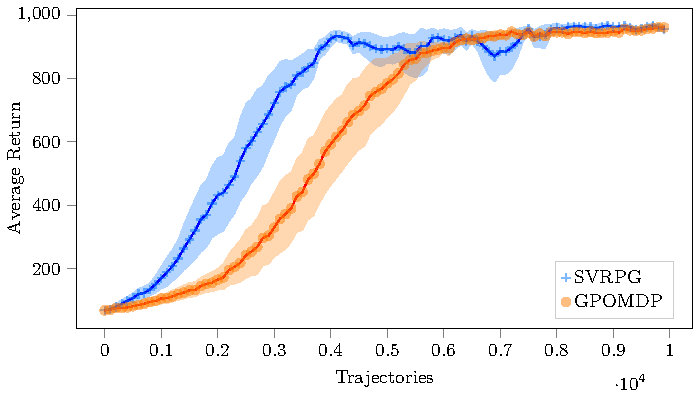
\includegraphics[width=.98\textwidth]{images/cartpole.pdf}};
	\node[above left] at ($(picture1.north west) + (2.7cm,-.6cm)$) {\textbf{Cart-Pole}};
\end{tikzpicture}%

\noindent
\begin{tikzpicture}
\node[inner sep=0pt] (picture2) {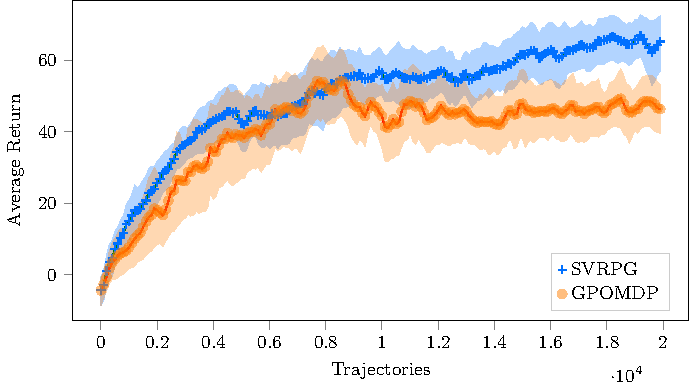
\includegraphics[width=0.98\textwidth]{images/swimmer.pdf}};
\node[above left] at ($(picture2.north west) + (2.8cm,-.5cm)$) {\textbf{Swimmer}};
\end{tikzpicture}%

\vspace*{-.3cm}

\noindent
\begin{tikzpicture}
\node[inner sep=0pt] (picture3) {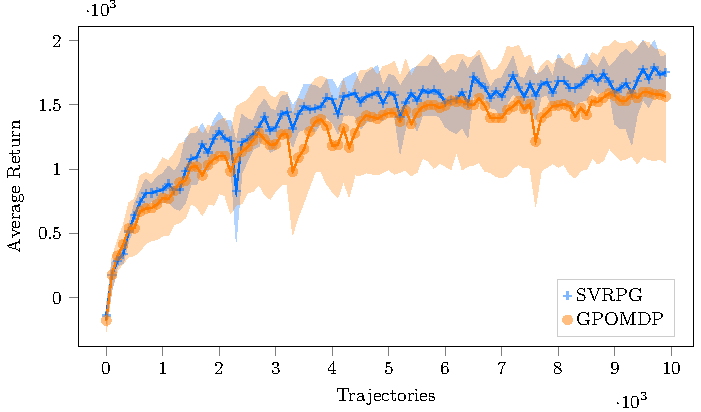
\includegraphics[width=0.98\textwidth]{images/cheetah.pdf}};
\node[above left] at ($(picture3.north west) + (3.4cm,-.8cm)$) {\textbf{Half-Cheetah}};
\end{tikzpicture}%
}

\headerbox{References}{name=ref,column=1,row=2,span=1,below=algo,above=bottom}{
        \tiny
\bibliographystyle{plainnat}
\begingroup
\renewcommand{\section}[2]{}%
\bibliography{poster.bib}
\endgroup
}


\end{poster}



\end{document}
